%!TEX root = proj.tex

\subsection{Weather data}\label{ch:desc_weather}
Historical weather data was obtained and prepared as described in \Cref{appx:weather_data_prep}. The preprocessed weather data is a more advanced time series containing several measurements for each time step. \Cref{tab:weather_data_attr} shows the attributes in the weather data set, and \Cref{tab:weather_data_example} shows an example of the data set.

\begin{table}[!ht]
    \center
    \begin{tabular}{p{.7in}p{4.5in}}        
        Attribute & Description \\
        \hline 
        \hline 
        \gls{t_i} & \glsdesc{t_i} \\
        \hline         
        \gls{temp_i} &  \glsdesc{temp_i}  \\
        \hline         
        \gls{pptn_i} & \glsdesc{pptn_i}\\
        \hline         
        \gls{rh_i} & \glsdesc{rh_i} \\
        \hline         
        \gls{ws_i} & \glsdesc{ws_i} \\
        \hline         
        \gls{cond_i} & \glsdesc{cond_i} \\
    \end{tabular}
    \caption{Attributes in the travel demand data set.}
    \label{tab:weather_data_attr}
\end{table}

\begin{table}[!ht]
    \center
    \begin{tabular}{lrrrrrll}
 Date/time & Temperature & Dew point & Wind speed & Humidity & Precipitation & Rain & Clear \\ 
  \hline
\hline
2016-10-01 00:00 & 12.00 & 10.00 & 24.10 &  78 & 0.00 & 0 & 0 \\ 
   \hline
2016-10-01 00:20 & 12.00 & 10.00 & 18.50 &  88 & 0.00 & 0 & 0 \\ 
   \hline
2016-10-01 00:50 & 12.00 & 10.00 & 16.70 &  88 & 0.00 & 0 & 0 \\ 
   \hline
2016-10-01 01:00 & 12.00 & 10.00 & 14.80 &  81 & 0.00 & 0 & 1 \\ 
   \hline
2016-10-01 01:20 & 12.00 & 10.00 & 13.00 &  88 & 0.00 & 0 & 0 \\ 
   \hline
2016-10-01 01:50 & 13.00 & 11.00 & 16.70 &  88 & 0.00 & 0 & 0 \\ 
   \hline
2016-10-01 02:00 & 13.00 & 11.00 & 20.40 &  85 & 0.00 & 0 & 0 \\ 
   \hline
2016-10-01 02:20 & 13.00 & 11.00 & 18.50 &  88 & 0.00 & 0 & 0 \\ 
   \hline
2016-10-01 02:50 & 12.00 & 10.00 & 14.80 &  88 & 0.00 & 0 & 0 \\ 
   \hline
2016-10-01 03:00 & 12.00 & 10.00 & 13.00 &  84 & 0.00 & 0 & 0 \\ 
  \end{tabular}

    \caption{Example of the weather data set.}
    \label{tab:weather_data_example}
\end{table}

Weather conditions seems quite sparse, e.g.\ as shown in \Cref{fig:weather_hist} rain conditions are only observed $\approx12 \%$ of the time, and show $<3 \%$ of the time. And in the vast majority of time it is raining the rain condition is considered \emph{light}.

\begin{figure}[!ht]
    \center
    % !TEX encoding = UTF-8 Unicode
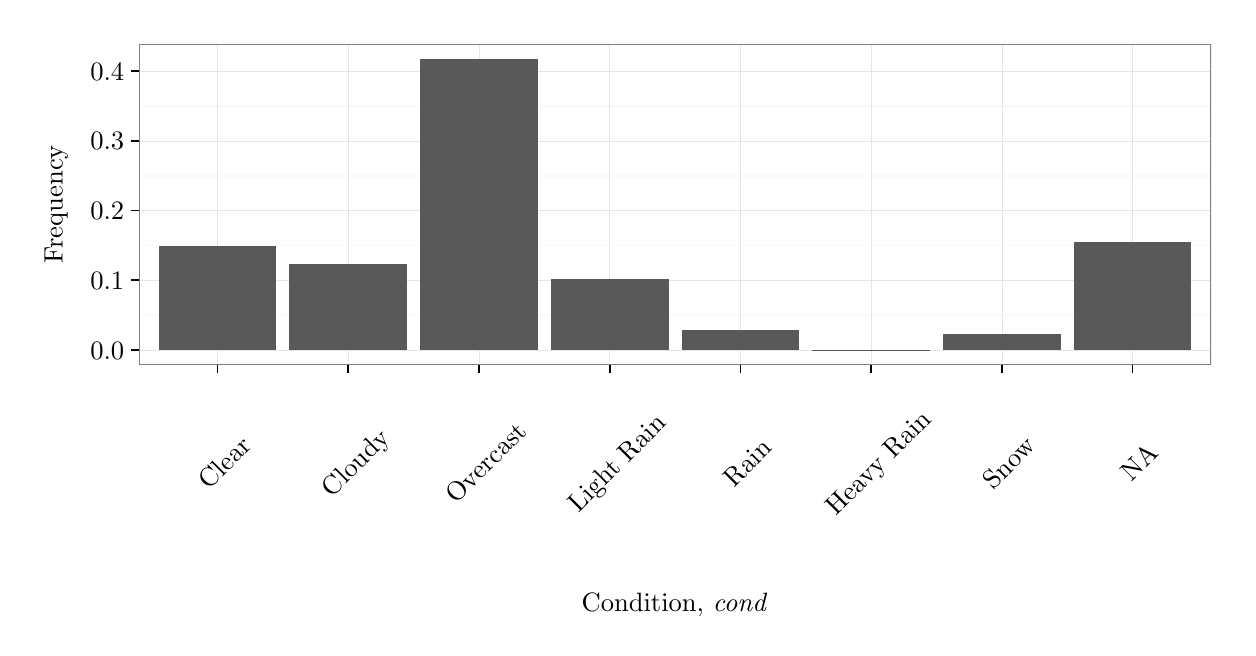
\begin{tikzpicture}[x=1pt,y=1pt]
\definecolor{fillColor}{RGB}{255,255,255}
\path[use as bounding box,fill=fillColor,fill opacity=0.00] (0,0) rectangle (433.62,216.81);
\begin{scope}
\path[clip] (  0.00,  0.00) rectangle (433.62,216.81);
\definecolor{drawColor}{RGB}{255,255,255}
\definecolor{fillColor}{RGB}{255,255,255}

\path[draw=drawColor,line width= 0.6pt,line join=round,line cap=round,fill=fillColor] (  0.00,  0.00) rectangle (433.62,216.81);
\end{scope}
\begin{scope}
\path[clip] ( 40.28, 95.07) rectangle (427.62,210.81);
\definecolor{fillColor}{RGB}{255,255,255}

\path[fill=fillColor] ( 40.28, 95.07) rectangle (427.62,210.81);
\definecolor{drawColor}{gray}{0.98}

\path[draw=drawColor,line width= 0.6pt,line join=round] ( 40.28,112.93) --
	(427.62,112.93);

\path[draw=drawColor,line width= 0.6pt,line join=round] ( 40.28,138.12) --
	(427.62,138.12);

\path[draw=drawColor,line width= 0.6pt,line join=round] ( 40.28,163.32) --
	(427.62,163.32);

\path[draw=drawColor,line width= 0.6pt,line join=round] ( 40.28,188.51) --
	(427.62,188.51);
\definecolor{drawColor}{gray}{0.90}

\path[draw=drawColor,line width= 0.2pt,line join=round] ( 40.28,100.33) --
	(427.62,100.33);

\path[draw=drawColor,line width= 0.2pt,line join=round] ( 40.28,125.52) --
	(427.62,125.52);

\path[draw=drawColor,line width= 0.2pt,line join=round] ( 40.28,150.72) --
	(427.62,150.72);

\path[draw=drawColor,line width= 0.2pt,line join=round] ( 40.28,175.91) --
	(427.62,175.91);

\path[draw=drawColor,line width= 0.2pt,line join=round] ( 40.28,201.11) --
	(427.62,201.11);

\path[draw=drawColor,line width= 0.2pt,line join=round] ( 68.62, 95.07) --
	( 68.62,210.81);

\path[draw=drawColor,line width= 0.2pt,line join=round] (115.85, 95.07) --
	(115.85,210.81);

\path[draw=drawColor,line width= 0.2pt,line join=round] (163.09, 95.07) --
	(163.09,210.81);

\path[draw=drawColor,line width= 0.2pt,line join=round] (210.33, 95.07) --
	(210.33,210.81);

\path[draw=drawColor,line width= 0.2pt,line join=round] (257.57, 95.07) --
	(257.57,210.81);

\path[draw=drawColor,line width= 0.2pt,line join=round] (304.80, 95.07) --
	(304.80,210.81);

\path[draw=drawColor,line width= 0.2pt,line join=round] (352.04, 95.07) --
	(352.04,210.81);

\path[draw=drawColor,line width= 0.2pt,line join=round] (399.28, 95.07) --
	(399.28,210.81);
\definecolor{fillColor}{gray}{0.35}

\path[fill=fillColor] ( 47.36,100.33) rectangle ( 89.87,137.96);

\path[fill=fillColor] ( 94.60,100.33) rectangle (137.11,131.52);

\path[fill=fillColor] (141.84,100.33) rectangle (184.35,205.55);

\path[fill=fillColor] (189.07,100.33) rectangle (231.59,126.12);

\path[fill=fillColor] (236.31,100.33) rectangle (278.82,107.52);

\path[fill=fillColor] (283.55,100.33) rectangle (326.06,100.45);

\path[fill=fillColor] (330.78,100.33) rectangle (373.30,106.11);

\path[fill=fillColor] (378.02,100.33) rectangle (420.53,139.35);
\definecolor{drawColor}{gray}{0.50}

\path[draw=drawColor,line width= 0.6pt,line join=round,line cap=round] ( 40.28, 95.07) rectangle (427.62,210.81);
\end{scope}
\begin{scope}
\path[clip] (  0.00,  0.00) rectangle (433.62,216.81);
\definecolor{drawColor}{RGB}{0,0,0}

\node[text=drawColor,anchor=base east,inner sep=0pt, outer sep=0pt, scale=  0.96] at ( 34.88, 97.02) {0.0};

\node[text=drawColor,anchor=base east,inner sep=0pt, outer sep=0pt, scale=  0.96] at ( 34.88,122.22) {0.1};

\node[text=drawColor,anchor=base east,inner sep=0pt, outer sep=0pt, scale=  0.96] at ( 34.88,147.41) {0.2};

\node[text=drawColor,anchor=base east,inner sep=0pt, outer sep=0pt, scale=  0.96] at ( 34.88,172.61) {0.3};

\node[text=drawColor,anchor=base east,inner sep=0pt, outer sep=0pt, scale=  0.96] at ( 34.88,197.80) {0.4};
\end{scope}
\begin{scope}
\path[clip] (  0.00,  0.00) rectangle (433.62,216.81);
\definecolor{drawColor}{RGB}{0,0,0}

\path[draw=drawColor,line width= 0.6pt,line join=round] ( 37.28,100.33) --
	( 40.28,100.33);

\path[draw=drawColor,line width= 0.6pt,line join=round] ( 37.28,125.52) --
	( 40.28,125.52);

\path[draw=drawColor,line width= 0.6pt,line join=round] ( 37.28,150.72) --
	( 40.28,150.72);

\path[draw=drawColor,line width= 0.6pt,line join=round] ( 37.28,175.91) --
	( 40.28,175.91);

\path[draw=drawColor,line width= 0.6pt,line join=round] ( 37.28,201.11) --
	( 40.28,201.11);
\end{scope}
\begin{scope}
\path[clip] (  0.00,  0.00) rectangle (433.62,216.81);
\definecolor{drawColor}{RGB}{0,0,0}

\path[draw=drawColor,line width= 0.6pt,line join=round] ( 68.62, 92.07) --
	( 68.62, 95.07);

\path[draw=drawColor,line width= 0.6pt,line join=round] (115.85, 92.07) --
	(115.85, 95.07);

\path[draw=drawColor,line width= 0.6pt,line join=round] (163.09, 92.07) --
	(163.09, 95.07);

\path[draw=drawColor,line width= 0.6pt,line join=round] (210.33, 92.07) --
	(210.33, 95.07);

\path[draw=drawColor,line width= 0.6pt,line join=round] (257.57, 92.07) --
	(257.57, 95.07);

\path[draw=drawColor,line width= 0.6pt,line join=round] (304.80, 92.07) --
	(304.80, 95.07);

\path[draw=drawColor,line width= 0.6pt,line join=round] (352.04, 92.07) --
	(352.04, 95.07);

\path[draw=drawColor,line width= 0.6pt,line join=round] (399.28, 92.07) --
	(399.28, 95.07);
\end{scope}
\begin{scope}
\path[clip] (  0.00,  0.00) rectangle (433.62,216.81);
\definecolor{drawColor}{RGB}{0,0,0}

\node[text=drawColor,rotate= 45.00,anchor=base,inner sep=0pt, outer sep=0pt, scale=  0.96] at ( 73.29, 57.39) {Clear};

\node[text=drawColor,rotate= 45.00,anchor=base,inner sep=0pt, outer sep=0pt, scale=  0.96] at (120.53, 57.39) {Cloudy};

\node[text=drawColor,rotate= 45.00,anchor=base,inner sep=0pt, outer sep=0pt, scale=  0.96] at (167.77, 57.39) {Overcast};

\node[text=drawColor,rotate= 45.00,anchor=base,inner sep=0pt, outer sep=0pt, scale=  0.96] at (215.00, 57.39) {Light Rain};

\node[text=drawColor,rotate= 45.00,anchor=base,inner sep=0pt, outer sep=0pt, scale=  0.96] at (262.24, 57.39) {Rain};

\node[text=drawColor,rotate= 45.00,anchor=base,inner sep=0pt, outer sep=0pt, scale=  0.96] at (309.48, 57.39) {Heavy Rain};

\node[text=drawColor,rotate= 45.00,anchor=base,inner sep=0pt, outer sep=0pt, scale=  0.96] at (356.72, 57.39) {Snow};

\node[text=drawColor,rotate= 45.00,anchor=base,inner sep=0pt, outer sep=0pt, scale=  0.96] at (403.95, 57.39) {NA};
\end{scope}
\begin{scope}
\path[clip] (  0.00,  0.00) rectangle (433.62,216.81);
\definecolor{drawColor}{RGB}{0,0,0}

\node[text=drawColor,anchor=base,inner sep=0pt, outer sep=0pt, scale=  0.96] at (233.95,  6.00) {Condition, $\mathit{cond}$};
\end{scope}
\begin{scope}
\path[clip] (  0.00,  0.00) rectangle (433.62,216.81);
\definecolor{drawColor}{RGB}{0,0,0}

\node[text=drawColor,rotate= 90.00,anchor=base,inner sep=0pt, outer sep=0pt, scale=  0.96] at ( 12.61,152.94) {Frequency};
\end{scope}
\end{tikzpicture}

    \caption{Frequency of different levels of rain.}
    \label{fig:weather_hist}
\end{figure}